\chapter{Détection d'objets et apprentissage profond}
\newpage
\pagestyle{fancy} 
\fancyhead[L]{\chaptername \ \thechapter}
\fancyhead[R]{Détection d'objets et apprentissage profond}
\renewcommand{\headrulewidth}{1pt}
\fancyfoot[C]{\thepage}
\section{Introduction} 
Malgré la popularité des techniques traditionnelles de vision par ordinateur et d'apprentissage automatique, le développement de l'apprentissage profond a renversé la situation, de sorte que de nombreux problèmes de vision par ordinateur y compris la détection d'objets se sont traités à l'aide d'architectures profondes, généralement des réseaux de neurones convolutifs (CNN) \cite{gupta2014learning}, qui ont pu surpasser les autres approches en termes d'efficience et d'efficacité.

Dans ce chapitre, nous allons introduire les réseaux de neurones convolutifs et exposer certains réseaux convolutifs communs qui sont souvent utilisés comme base pour les systèmes de détection d'objets, et les techniques courantes d'apprentissage telles que l'apprentissage par transfert.

Également, nous présenterons  les différentes bases d'images et métriques utilisées pour l'évaluation. En outre, nous décrirons certaines des méthodes basées sur l'apprentissage profond existantes. 



% =========== CNN =========== 
\section{Les réseaux de neurones convolutifs } 

Un réseau de neurones convolutif (CNN ou ConvNet) est un type de réseau de neurones artificiels acyclique  dans lequel l'architecture des connexions est inspirée de celle du cortex visuel des mammifères \cite{Deep2018}.
 
Un réseau de neurones convolutif  est  distingué des réseaux de neurones classiques entièrement connectés en combinant un certain nombre de couches connectées localement destinées à l'extraction automatique des caractéristiques, suivies d'un nombre de couches entièrement connectées destinées à la classification \cite{Deep2016}.

 Un CNN comprend une succession de couches pour extraire les caractéristiques discriminante, plusieurs couches distinctes,chacune ayant un objectif spécifique, notamment  des couches convolutives, de correction,  des couches de sous-échantillonnage appelées couches de pooling, des couches entièrement connectées. La façon dont s'enchaînent ces couches font la caractéristique de l'architecture du réseau. Ces couches sont décrites brièvement dans les sous-sections suivantes:

\begin{enumerate}
\item \underline{\textbf{La couche de convolution :}}
Une couche de convolution est un empilement de convolutions. En effet, l'image est parcourue par plusieurs noyaux de convolution permettant d'extraire des entités d'une image d'entrée. Trois hyperparamètres qui permettent de préciser le volume de la couche de convolution :  profondeur, pas et  marge \cite{CNN2015}.  

\begin{itemize}
\item \textbf{Profondeur de la couche:} nombre de noyaux de convolution (ou nombre de neurones associés à un même champ récepteur).

 \item \textbf{Le pas:} contrôle le chevauchement des champs récepteurs. Plus le pas est petit, plus les champs récepteurs se chevauchent et plus le volume de sortie est élevé.
  
 \item  \textbf{La marge (à 0) ou zéro remplissage:} est le processus simple de remplissage de la bordure de l'entrée, elle constitue une méthode efficace pour mieux contrôler la dimensionnalité des volumes de sortie.

\end{itemize}
Tout simplement, La convolution est une opération mathématique simple généralement utilisée pour le traitement et la reconnaissance d'images. Sur une image, son effet s'assimile à un filtrage,  dont fonctionnement est présenté dans la figure \ref{conv}

\begin{figure}[H]
\centering
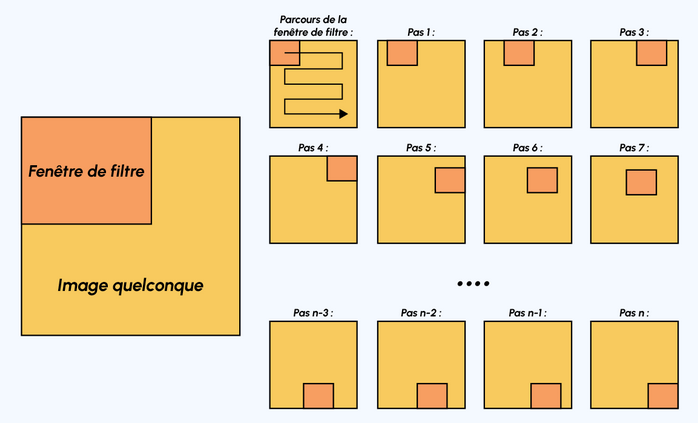
\includegraphics[height=6cm,width=12cm]{Chapitre2/conv.png}
\caption{Principe d'une convolution d'image.}
\label{conv}
\end{figure}

À chaque portion d'image rencontrée, une convolution s'effectue permettant d'obtenir en sortie une \textbf{carte d'activation ou de caractéristiques} ou \textbf{feature map} qui indique où sont localisées les caractéristiques dans l'image. 

\item \underline{\textbf{La couche de pooling:}}
C'est une technique de sous-échantillonnage. Généralement, une couche de pooling est insérée régulièrement entre deux couches convolutives successives.  Cela permet de réduire la taille spatiale des cartes de caractéristiques, donc le nombre de paramètres du réseau, ce qui accélère le temps de calcul et contrôle le risque de sur-apprentissage. 
Les trois types d'opérations de pooling sont :
\begin{itemize}
\item Le max pooling : la valeur de pixel maximale de la partie de l'image couverte par la fenêtre du filtre est renvoyée (voir figure \ref{pool}).
\item Le min pooling : La valeur de pixel minimale  de la partie de l'image couverte par la fenêtre du filtre est renvoyée.
\item Average pooling : la valeur moyenne de tous les pixels  de la partie de l'image couverte par la fenêtre du filtre est renvoyée(voir figure \ref{pool}).
\end{itemize}
 
     \begin{figure}[H]
          \centering
          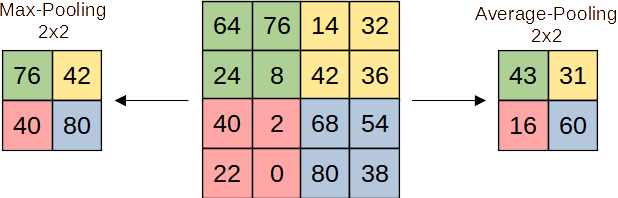
\includegraphics[height=5cm,width=15cm]{Chapitre2/img3.png}
          \caption{Max-pooling et Average-pooling.}
          \label{pool}
          \end{figure}

Les trois opérations de pooling sont illustrées dans la figure \ref{poolef}

\begin{figure}[H]
\centering
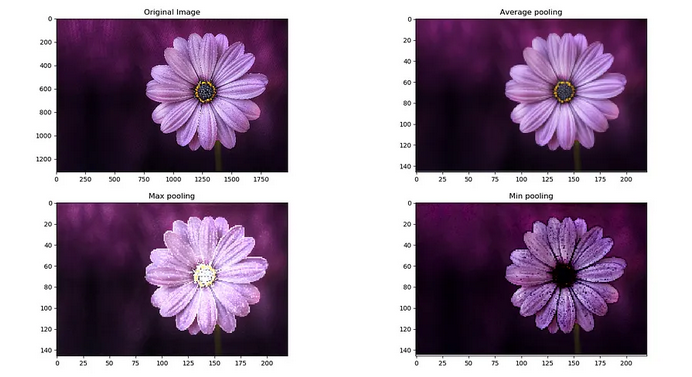
\includegraphics[height=5.5cm,width=11cm]{Chapitre2/poolef.png}
\caption{Average, Max and Min pooling de taille 9 x 9 appliqués à une image.}
\label{poolef}
\end{figure}

\item \underline{\textbf{La couche de correction (ReLu) :}}
La couche de correction est l'application d'une fonction non-linéaire(voir la figure \ref{relu} aux sorties de la couche de convolution, où toutes les valeurs de pixels négatifs sont mises à zéro. Le but est d'introduire la non-linéarité dans le CNN, ce qui permet de faciliter l'extraction des caractéristiques complexes qui ne peuvent pas être modélisées par une combinaison linéaire.

\begin{figure}[H]
\centering
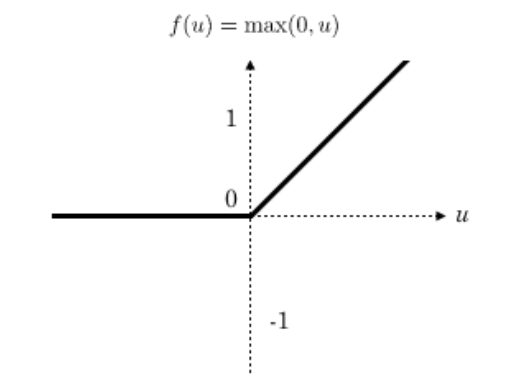
\includegraphics[height=4.5cm,width=6cm]{Chapitre2/relu.png}
\caption{La fonction ReLu.}
\label{relu}
\end{figure}

\item \underline{\textbf{La couche entièrement connectée(FC):}}
La couche entièrement connectée est un perceptron multicouche traditionnel (Multi Layer Perceptron) utilisant une fonction d'activation notamment appelée softmax dans la couche de sortie. 

Elle est entièrement connectée, car chaque neurone dans la couche précédente est connecté à chaque neurone sur la couche suivante. La couche entièrement connectée utilise ses sorties pour classer l'image d'entrée dans différentes classes en fonction de l'ensemble de données d'apprentissage \cite{CNN2015}.  
\end{enumerate}     
     % =========== Fully Connected Layer ===========
La figure \ref{img4} montre un exemple d'une structure d'un réseau de neurones convolutif:
     \begin{figure}[H]
          \centering
          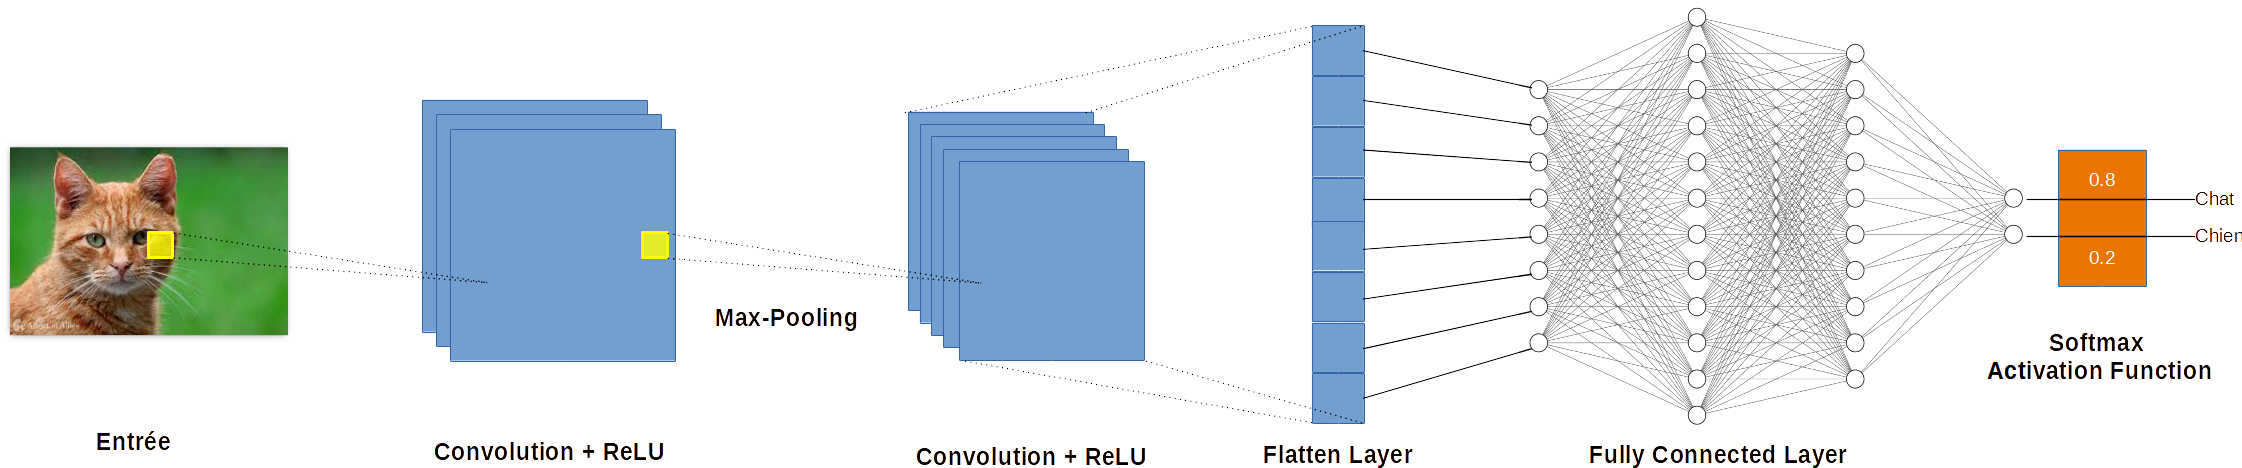
\includegraphics[height=4cm,width=18cm]{Chapitre2/img4.png}
          \caption{Exemple de structure de réseaux de neurones convolutif.}
          \label{img4}
          \end{figure}

% =========== Transfer Learning ===========
     \subsection{L'apprentissage par transfert} 
     L'apprentissage par transfert se produit lorsque des modèles existants sont réutilisés pour résoudre un nouveau défi ou problème. L'apprentissage par transfert n'est pas un type distinct d'algorithme d'apprentissage automatique, mais plutôt une technique ou une méthode utilisée lors de l'entraînement des modèles. Les connaissances acquises lors des entraînements précédents sont recyclées pour aider à effectuer une nouvelle tâche. La nouvelle tâche sera liée d'une certaine manière à la tâche précédemment entraînée.

     Le processus prend des parties pertinentes d'un modèle existant et les applique pour résoudre un problème nouveau mais similaire. Un élément clé de l'apprentissage par transfert est la généralisation. Cela signifie que seules les connaissances pouvant être utilisées par un autre modèle dans différents scénarios ou conditions sont transférées. Au lieu que les modèles soient liés de manière rigide à un ensemble de données d'entraînement, les modèles utilisés dans l'apprentissage par transfert seront plus généralisés. Les modèles développés de cette manière peuvent être utilisés dans des conditions changeantes et avec différents ensembles de données.
     \begin{figure}[H]
          \centering
          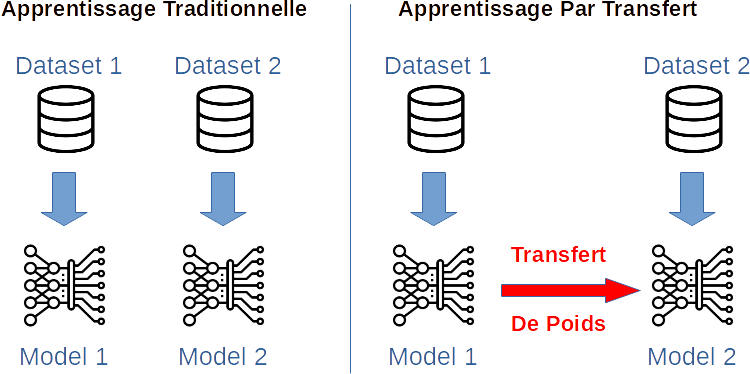
\includegraphics[height=7cm,width=13cm]{Chapitre2/img5.png}
          \caption{Différence entre l'apprentissage traditionnel et l'apprentissage par transfert.}
          \label{img5}
          \end{figure}

% =========== Backbones =========== 
\section{Architectures de réseau profond populaires} 
Certains réseaux profonds ont apporté des contributions si importantes dans le domaine qu'ils sont devenus des normes largement connues. C'est le cas d'AlexNet, VGG-16, GoogLeNet et ResNet. Leur importance était telle qu'ils sont actuellement utilisés comme éléments de base pour de nombreuses architectures de détection d'objets. Pour cette raison, nous consacrerons cette section à leur présentation. 

\begin{enumerate}
\item \textbf{AlexNet}\cite{alexnet}\\
AlexNet a été le  CNN pionnier qui a largement surpassé ses concurrents au défi ImageNet ILSVRC-2012 avec une précision de test TOP-5 de 84,6\% tandis que le concurrent le plus proche, qui utilisait des techniques traditionnelles au lieu d'architectures profondes, a atteint une précision de 73,8\% dans le même défi. L'architecture présentée par Krizhevsky et coll. était relativement simple, elle est composée de huit couches d'entraînement, cinq couches de convolution et trois couches entièrement connectées. Toutes les couches entraînables sont suivies d'une fonction d'activation (ReLu) à l'exception de la dernière couche entièrement connectée où une fonction softmax est utilisée. L'architecture aussi se compose de couches
non entraînables : trois couches de pooling, deux couches de normalisation et une couche Dropout. cette architecture est clairement présentée sur la figure\ref{alexnet}.

\begin{figure}[H]
\centering
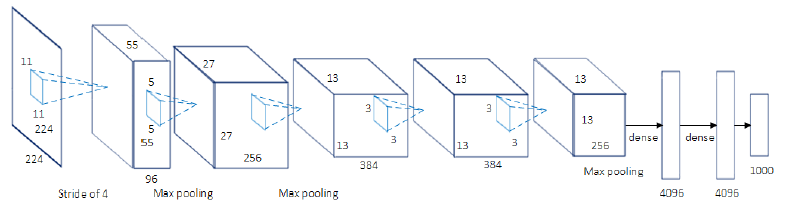
\includegraphics[height=2in,width=6in]{Chapitre2/alexnet.png}
\caption{Architecture du réseau convolutif AlexNet. \cite{alexnet}}
\label{alexnet}
\end{figure} 
\item \textbf{VGG}\cite{vgg}\\
Visual Geometry Group (VGG) est un modèle CNN introduit par le Groupe de Géométrie Visuelle (VGG) de l'Université d'Oxford. Ils ont proposé divers modèles et configurations de CNN profonds, l'un d'eux a été soumis au ImageNet Large Scale Visual Recognition Challenge (ILSVRC)-2013. Ce modèle, également connu sous le nom de VGG-16 , est devenu populaire grâce à sa précision  de test TOP-5 de 92,7\% . 
La figure \ref{vgg} montre la configuration de VGG-16. La principale différence entre VGG - 16 et ses prédécesseurs est l'utilisation d'un empilement de couches de convolution avec de petits champs réceptifs  dans les premières couches au lieu de quelques couches avec grands champs réceptifs. Cela conduit à moins de paramètres et plus de non-linéarités entre les deux, rendant ainsi la fonction de décision plus discriminante et le modèle plus facile à entraîner.
\begin{figure}[H]
\centering
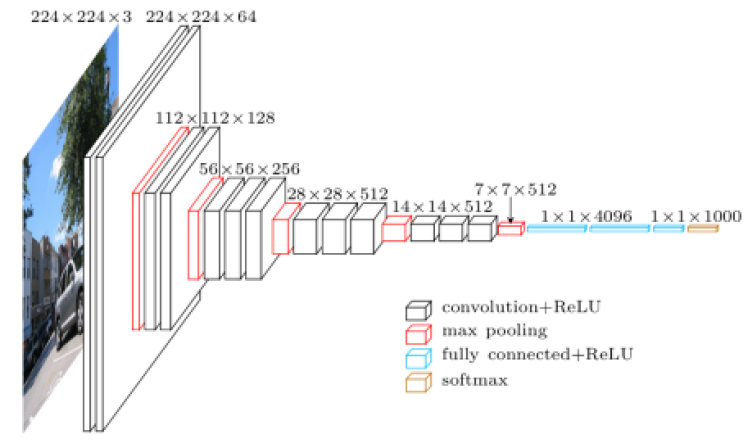
\includegraphics[height=2in,width=6in]{Chapitre2/vgg.png}
\caption{Architecture du réseau convolutif VGG-16. }
\label{vgg}
\end{figure} 
\item \textbf{GoogleNet}\cite{google}\\
En 2014, les chercheurs de Google ont présenté le réseau GoogLeNet, qui a pris la première place du concours ImageNet en 2014 pour les défis de classification et de détection. La principale caractéristique intéressante de GoogLeNet est qu'il fonctionne très rapidement en raison de l'introduction d'un nouveau concept appelé (inception module), il est clairement illustré sur la figure \ref{google}. Ce module est basé sur plusieurs très petites convolutions afin de réduire drastiquement le nombre de paramètres à seulement 5 millions ; c'est 12 fois moins qu'AlexNet. Il utilise moins de mémoire et moins d'énergie. L'architecture GoogLeNet se compose de 22 couches.GoogLeNet est principalement utilisé dans le modèle de détection d'objets YOLO.
\begin{figure}[H]
 \centering
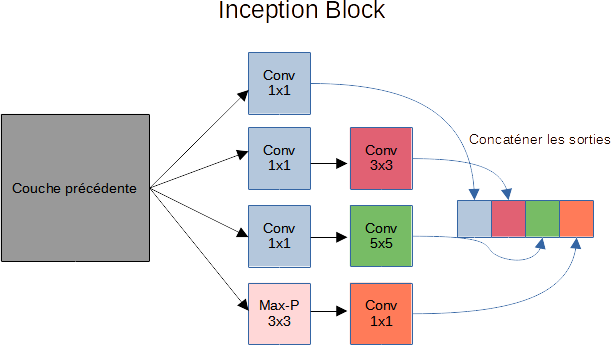
\includegraphics[height=8cm,width=12cm]{Chapitre2/img9.png}
\caption{Structure de Inception Block.}
 \label{img9}
 \end{figure}

\item \textbf{ResNet}\cite{resnet}\\
Les réseaux résiduels profonds (ResNet) sont basés sur l'idée de développer des réseaux beaucoup plus profonds (des centaines de couches par opposition à des dizaines de couches). Dans ResNets, les couches de convolution sont divisées en blocs résiduels (voir figure \ref{resnet}), et pour chaque bloc, une connexion résiduelle est ajoutée, qui contourne le bloc correspondant. Ensuite, la sortie du bloc résiduel est additionnée avec l'entrée d'origine passée à travers la connexion résiduelle. 
\begin{figure}[H]
\centering
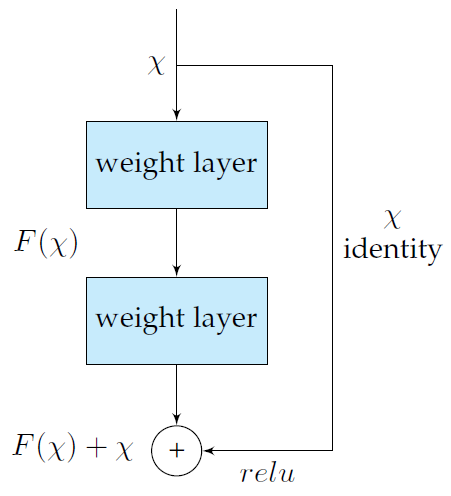
\includegraphics[height=2in,width=2.5in]{Chapitre2/resnet.png}
\caption{ Bloc résiduel de l'architecture ResNet. \cite{resnet}}
\label{resnet}
\end{figure} 

\item \textbf{SqueezeNet} \cite{SqueezeNet2016}
Une petite architecture CNN avec une précision équivalente à AlexNet. Ça peut être  3 fois plus rapide et 500 fois plus petit qu'AlexNet.
Il est construit sur une architecture spécifique, que l'on appelle (Fire module) qui contient une couche de compression(Squeeze) et une couche d'extension (expand), il est clairement illustré sur la figure \ref{SN}.

Les couches de compression(Squeeze) sont des couches de convolution composées uniquement de filtres $1\times 1$ et les couches d'extension sont des couches de convolution avec un mélange de filtres $1 \times 1$ et $3 \times 3$.
\begin{figure}[H]
\centering
  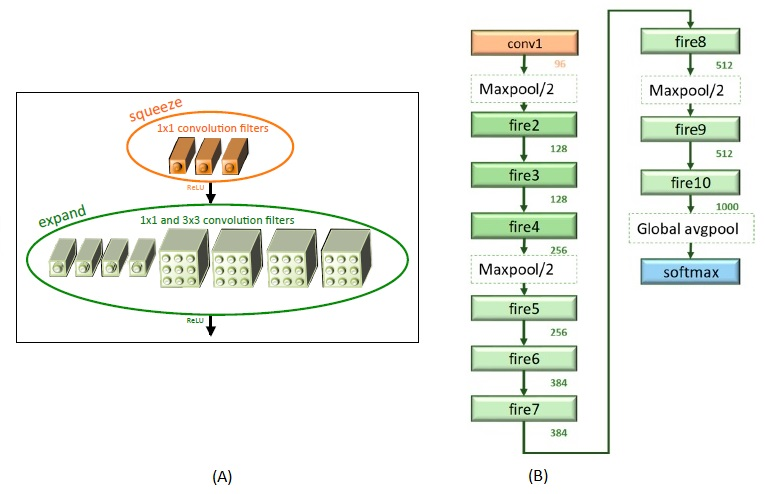
\includegraphics[width=9cm, height=7cm]{Chapitre2/SN.jpg} 
   \caption{(A) Fire module (B)Architecture de SqueezeNet \cite{SqueezeNet2016}.}
   \label{SN}
 \end{figure}

\item \textbf{ShuffleNet} \cite{shufflenet2018} et \textbf{ShuffleNetV2}\cite{shufflenetV2}
Une architecture CNN très efficace en termes de calcul, conçue principalement pour les appareils mobiles avec une puissance de calcul limitée. L'architecture introduit deux opérations clés pour réduire considérablement les coûts de calcul tout en conservant la précision. La première opération consiste en des convolutions de groupe par points (pointwise group convolutions), qui peuvent réduire la complexité de calcul des convolutions 1 × 1. Néanmoins, ces convolutions ont un effet secondaire, qui fait que les outputs d'un canal en particulier ne sont dérivées que d'une petite fraction des canaux d'input. Cet effet peut être diminué en divisant les canaux de chaque groupe en de multiples sous-groupes, ce qui est l'opération de mélange de canaux (channel shuffle).

ShuffleNetV2 propose de nombreux guides pratiques pour des architectures CNN efficientes. Il optimise davantage l’architecture avec des changements dans le goulot d’étranglement et en présentant la division de canaux (channel split). La figure montre clairement les différences entre ShuffleNet (a., b.) et ShuffleNetV2 (c. d.).

\begin{figure}[H]
\centering
  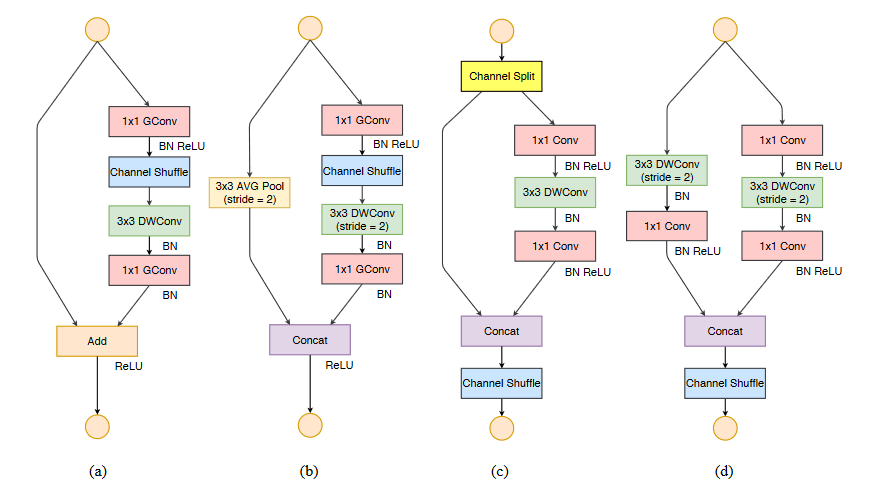
\includegraphics[width=17cm, height=7cm]{Chapitre2/shuffle.png} 
   \caption{Les unités de construction de l'architecture ShuffleNet  \cite{shufflenet2018} et ShuffleNetV2\cite{shufflenetV2}.}
   \label{shuffle}
 \end{figure}
 
\item \textbf{MobileNetV2 } \cite{mobilenetv2}
La version deux des séries MobileNet introduit les résiduels inversés (inverted residuals) et les goulots d'étranglement linéaires (linear bottlenecks) pour améliorer les performances de MobileNets. Les résiduels inversés permettent au réseau de calculer des activations (ReLU) de manière plus efficace, et de maintenir plus d’informations après activation. La figure \ref{mobv2} montre le goulot d'étranglement, et inclue les résiduels inversés. Sur ce schéma, les blocs plus épais ont plus de canaux. 

\begin{figure}[H]
\centering
  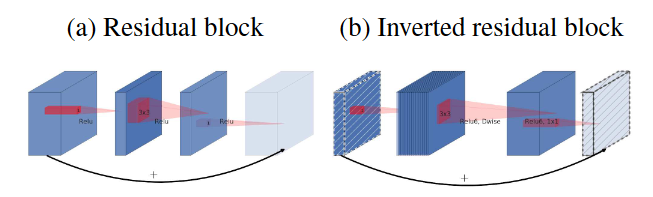
\includegraphics[width=10cm, height=5cm]{Chapitre2/mobv2.png} 
   \caption{La différence entre bloc résiduel \cite{mobilenet}
et résiduel inversé \cite{mobilenetv2}.}
   \label{mobv2}
 \end{figure}
 
\item \textbf{Darknet-53} \cite{yolov3_paper}
Introduit en 2018 Darknet-53 par Joseph Redmon Ali Farhadi, c'est un réseau neuronal convolutif qui sert de base pour l'extraction de caractéristiques dans l'approche de détection d'objets YOLOv3. C'est une amélioration de son prédécesseur Darknet-19 sur lequel est basé l'architecture de YOLOv2.
Les améliorations par rapport à Darknet-19 incluent l'utilisation de connexions résiduelles, ainsi que davantage de couches.

L'architecture du réseau Darknet-53 est illustrée à la figure \ref{img10}. Ce modèle de réseau combine les blocs résiduels et le réseau d'extraction de caractéristiques de base YOLOv2, Darknet-19 \cite{yolov3_paper}, en utilisant des couches de convolution et des blocs résiduels successifs $1\times 1$ et $3\times 3$. La couche convolutive, la couche de normalisation par lots et la couche Leaky Relu constituent ensemble sa plus petite composante.

           \begin{figure}[H]
                \centering
                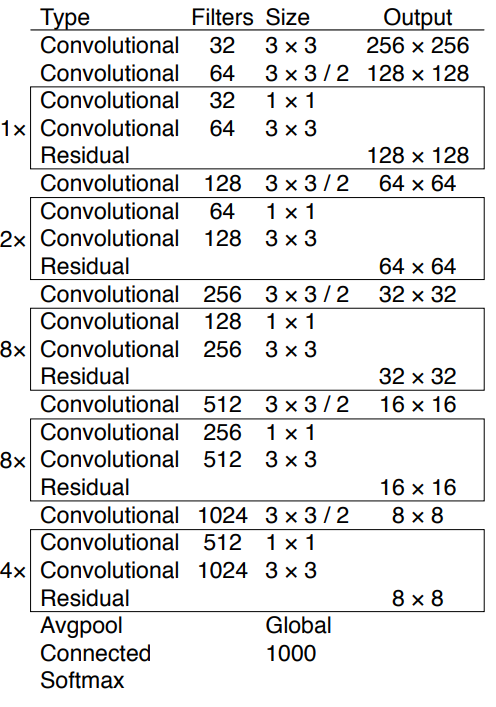
\includegraphics[height=9cm,width=8cm]{Chapitre2/img10.png}
                \caption{Architecture du réseau Darknet-53 \cite{yolov3_paper}.}
                \label{img10}
                \end{figure}

Notez que le classificateur en bas n'est utilisé que lors de l'utilisation du réseau pour la classification d'objets plutôt que pour la localisation d'objets. 

\end{enumerate}


     
          % =========== AlexNet =========== 

          % =========== VGG-16 ===========


          % =========== ResNet ===========
          
          % =========== GoogLeNet ===========

           % =========== Darknet-53 ===========





\section{Les méthodes de détections d'objets basées sur l'apprentissage profond}
Comme nous avons déjà mentionné dans le chapitre précédent, la détection d'objets basée sur l'apprentissage profond est regroupée en deux classes : la "détection en deux étapes" et la "détection en une étape".

En général, les détecteurs d'objets basés sur l'apprentissage en profondeur extraient des caractéristiques de l'image d'entrée. Un détecteur d'objets résout deux tâches successives :
\begin{itemize}
\item  Tâche n° 1 : trouver un nombre arbitraire d'objets (peut-être même zéro), et
\item  Tâche n° 2 : classer chaque objet et estimer sa taille à l'aide d'un cadre englobant.
\end{itemize}

Pour simplifier le processus, on peut séparer ces tâches en deux étapes. D'autres méthodes combinent les deux tâches en une seule étape (détecteurs à une étape) pour obtenir des performances plus élevées au détriment de la précision.

% =========== Two-Stage ===========
\subsection{La détection d'objets en deux étapes}
 
Dans les détecteurs d'objets à deux étages, les régions d'objet approximatives sont proposées à l'aide de caractéristiques profondes avant que ces caractéristiques ne soient utilisées pour la classification.

     L'architecture en deux étapes implique une proposition de région d'objet avec des méthodes conventionnelles de vision par ordinateur ou des réseaux profonds, suivie d'une classification d'objet basée sur des caractéristiques extraites de la région proposée.   
     Ces méthodes permettent d'obtenir une précision de détection  plus élevée, mais sont généralement plus lentes. 
     
    
     % =========== RCNN ===========
\subsubsection{Les modèles R-CNN}  
La famille de méthodes R-CNN fait référence au R-CNN, qui peut signifier "Régions avec des caractéristiques CNN" ou "Réseau de neurones convolutifs basés sur les régions", développé par Ross Girshick, et al.

Cela inclut les techniques R-CNN, Fast R-CNN et Faster-RCNN conçues et démontrées pour la localisation et la reconnaissance d'objets.

\begin{enumerate}
 \item  \textbf{R-CNN}\cite{rcnn_paper}
 
Le R-CNN a été introduit par Ross Girshick et al en 2004. Il s'agit peut-être de l'une des premières applications importantes des réseaux de neurones convolutifs au problème de la localisation, de la détection et de la segmentation d'objets. Le modèle R-CNN proposé est composé de trois modules qui sont:
\begin{itemize}
\item \underline{Module 1 : Proposition de Région.} Générez et extrayez des propositions de régions indépendantes des catégories, par ex. boîtes englobantes candidates.
\item \underline{Module 2 : Extracteur de caractéristiques.} Extraire une caractéristique de chaque région candidate, par ex. à l'aide d'un réseau de neurones à convolution profonde.
\item \underline{Module 3 : Classificateur.} Classer les caractéristiques comme faisant partie de la classe connue, par ex. modèle de classificateur SVM linéaire.
\end{itemize}
 
L'architecture du modèle est résumée dans l'image ci-dessous.
 \begin{figure}[H]
          \centering
          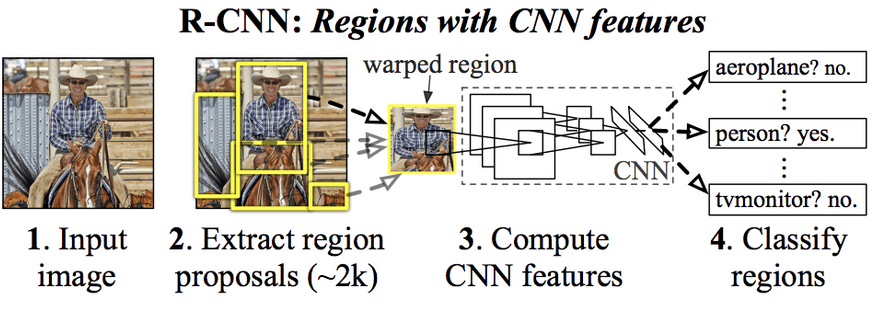
\includegraphics[height=6cm,width=15cm]{Chapitre2/img11.png}
          \caption{Architecture d'un R-CNN \cite{rcnn_paper}}
          \label{img11}
          \end{figure}

Une Recherche sélective qui est une technique de vision par ordinateur est utilisée pour proposer des régions candidates ou des boîtes englobantes d'objets potentiels dans l'image, bien que la flexibilité de la conception permette d'utiliser d'autres algorithmes de proposition de région.

L'extracteur de caractéristiques utilisé par le modèle est le modèle AlexNet. La sortie du CNN est un vecteur de 4 096 éléments qui décrit le contenu de l'image. Ce dernier est transmis à un SVM linéaire pour la classification, en particulier un SVM est entraîné pour chaque classe connue.

Il s'agit d'une application relativement simple et directe des CNN au problème de la localisation et de la reconnaissance d'objets. Un inconvénient de l'approche est qu'elle est lente, nécessitant une phase d'extraction de caractéristiques basée sur un CNN sur chacune des régions candidates générées par l'algorithme de proposition de région. C'est un vrai problème car le document initiale décrit le modèle fonctionnant sur environ 2 000 régions proposées par image au moment du test.
          
 \item  \textbf{Fast R-CNN}\cite{fast_rcnn_paper}
 
Fast R-CNN a été proposé par Ross Girshick en 2015 comme extension aux R-CNN  pour résoudre les problèmes de vitesse.

Fast R-CNN est proposé comme un modèle unique au lieu d'un pipeline pour apprendre et produire directement des régions et des classifications.

L'architecture du modèle prend l'image comme entrée d'un ensemble de propositions de régions qui sont transmises à travers un réseau de neurones convolutif. Un CNN pré-entraîné, tel qu'un VGG-16, est utilisé pour l'extraction de caractéristiques. La sortie du CNN est une couche personnalisée appelée couche de regroupement de régions d'intérêt, ou regroupement RoI (Region of Interest Pooling Layer, or RoI Pooling), qui extrait des caractéristiques spécifiques à une région candidate d'entrée donnée. 

La sortie du CNN est ensuite interprétée par une couche entièrement connectée, puis le modèle se divise en deux sorties, une pour la prédiction de classe via une couche softmax, et une autre avec une sortie linéaire pour la boîte englobante. Ce processus est ensuite répété plusieurs fois pour chaque région d'intérêt dans une image donnée.

L'architecture du modèle est résumée dans l'image \ref{img13}

\begin{figure}[H]
          \centering
          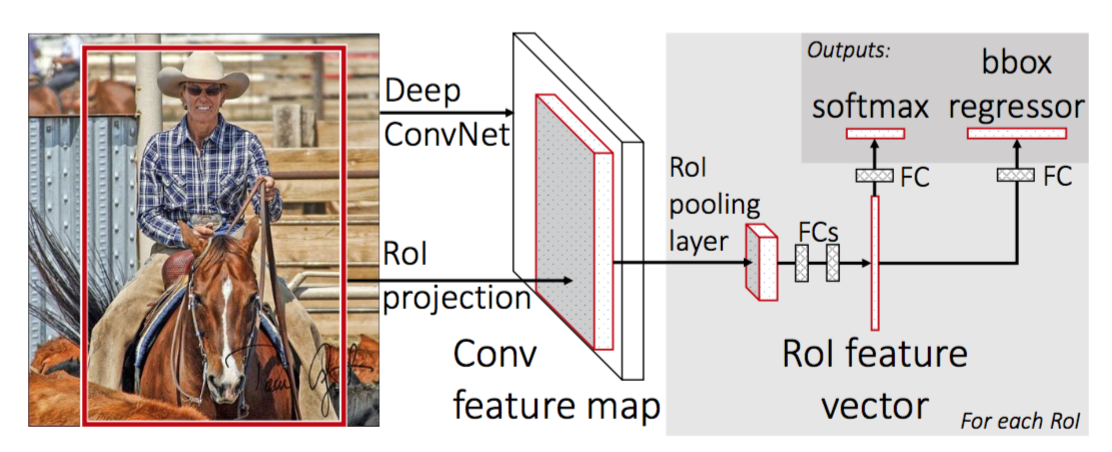
\includegraphics[height=5cm,width=15cm]{Chapitre2/img13.png}
          \caption{Architecture d'un Fast-RCNN \cite{fast_rcnn_paper}}
          \label{img13}
          \end{figure}

Le modèle est beaucoup plus rapide à entraîner et à faire des prédictions, mais nécessite toujours qu'un ensemble de régions candidates soit proposé avec chaque image d'entrée.

 \item  \textbf{Faster R-CNN}\cite{faster_rcnn_paper}
 
Proposée par Shaoqing Ren, et al. en 2016, toujours dans le but d'améliorer la vitesse d'entraînement et de détection des modèles précédemment décrits.

L'architecture a été conçue à la fois pour proposer et affiner les propositions de région dans le cadre du processus d'entraînement, appelé Réseau de proposition de régions, ou RPN. Ces régions sont ensuite utilisées parallèlement avec un modèle Fast R-CNN dans une conception de modèle unique. Ces améliorations réduisent à la fois le nombre de propositions de régions et accélèrent le fonctionnement en temps de test du modèle.

Bien qu'il s'agit d'un seul modèle unifié, l'architecture est composée de deux modules :
\begin{itemize}
\item \underline{Module 1 : Réseau de proposition de région.}  Réseau de neurones convolutifs pour proposer des régions et le type d'objet à considérer dans la région.
\item \underline{Module 2 : R-CNN rapide.} Réseau neuronal convolutif pour extraire les caractéristiques des régions proposées et produire la boîte englobante et les étiquettes de classe.
\end{itemize}

Les deux modules fonctionnent sur la même sortie d'un CNN profond. Le réseau de proposition de région agit comme un mécanisme d'attention pour le réseau Fast R-CNN, informant le deuxième réseau de l'endroit où regarder ou prêter attention.

L'architecture du modèle est résumée dans l'image \ref{img14}:

\begin{figure}[H]
          \centering
          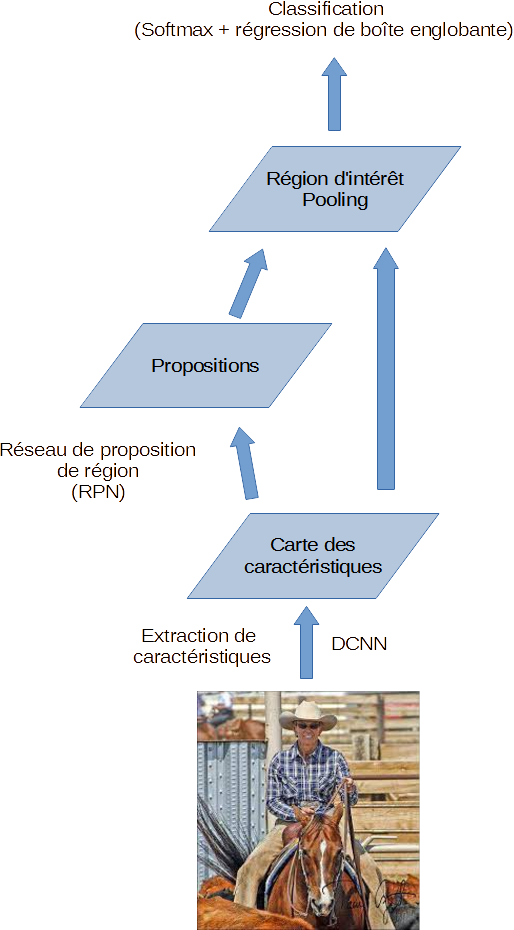
\includegraphics[height=13cm,width=8cm]{Chapitre2/img14.png}
          \caption{Architecture d'un Faster-RCNN}
          \label{img14}
          \end{figure}
          
Le RPN fonctionne en prenant la sortie d'un CNN profond pré-entraîné, tel que VGG-16, et en passant un petit réseau sur la carte des caractéristiques et en produisant plusieurs propositions de régions et une prédiction de classe pour chacune. Les propositions de régions sont des boîtes englobantes, basées sur des boîtes dites d'ancrage ou des formes prédéfinies conçues pour accélérer et améliorer la proposition de régions. La prédiction de classe est binaire, indiquant la présence d'un objet, ou non.

Une procédure d'apprentissage alterné est utilisée où les deux sous-réseaux sont entraînés en même temps. Cela permet aux paramètres du CNN profond du détecteur de caractéristiques d'être adaptés ou affinés pour les deux tâches en même temps.
 \end{enumerate} 


     % =========== Fast-RCNN ===========
    
     % =========== Faster-RCNN ===========
     
% =========== One-Stage ===========
\subsection{La détection d'objets en une étape}
Contrairement aux détecteurs à deux étapes, ces modèles ignorent l'étape de proposition de région des modèles à deux étages et exécutent la détection directement sur un échantillonnage dense d'emplacements. Ils considèrent généralement toutes les positions sur l'image comme des objets potentiels et essaient de classer chaque région d'intérêt comme arrière-plan ou comme objet cible.

     % =========== YOLO ===========
\subsubsection{YOLO (You Only Look Once) \cite{yolo_paper} }

Le modèle a été décrit pour la première fois par Joseph Redmon et al. en 2015. 
L'approche implique un seul réseau neuronal entraîné de bout en bout qui prend une image en entrée et prédit directement les boîtes englobantes et les étiquettes de classe pour chaque boîte englobante. La technique offre une précision prédictive inférieure (par exemple, plus d'erreurs de localisation), bien qu'elle fonctionne à 45 images par seconde et jusqu'à 155 images par seconde pour une version optimisée en vitesse du modèle.

En outre, YOLO sélectionne GoogLeNet comme réseau de base. Il se compose de 24 couches convolutives et de 2 couches entièrement connectées avec une entrée réseau de 448 × 448 images. Il divise l'image complète en grilles S×S. Chaque cellule de grille est responsable de la détection du centre de l'objet tombant dans la cellule de grille. Chaque cellule de la grille prédit les probabilités de classe C, les boîtes englobantes B et les scores de confiance, et l'image complète est codée pour produire le tenseur SxSx(5B+C).
     \begin{figure}[H]
          \centering
          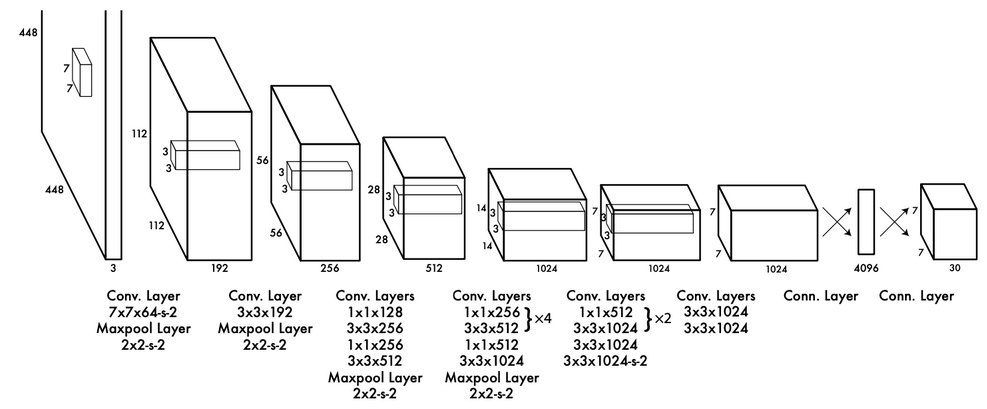
\includegraphics[height=7cm,width=16cm]{Chapitre2/img151.png}
          \caption{Architecture de YOLO (You Only Look Once)}
          \label{img15}
          \end{figure}

     % =========== YOLOv3 ===========
\subsubsection{YOLOv3 \cite{yolov3_paper}} 

Proposé par Redmon J et Farhadi deux ans plus tard en 2018 après la première version de YOLO. c'est une version améliorée de YOLO et YOLOv2. Il existe des différences majeures entre YOLOv3 et les anciennes versions en termes de vitesse, de précision et de spécificité des classes. YOLOv2 utilise Darknet-19 comme extracteur de caractéristiques de base, tandis que YOLOv3 utilise Darknet-53.    
    
Darknet-53  combine des blocs résiduels et FPN (Feature Pyramid Network). C'est un extracteur de caractéristiques qui prend une image à échelle unique d'une taille arbitraire en entrée et des sorties proportionnellement dimensionnées cartes de fonctionnalités à plusieurs niveaux, ce qui donne de bonnes performances sur une large gamme de résolutions d'entrée.

Darknet-53  est plus puissant que le Darknet-19 et plus efficace que les backbones concurrents (ResNet-101 ou ResNet-152). Il est également rapide et précis en termes de précision moyenne moyenne (mAP) et de valeurs d'intersection sur l'union (IOU). Il fonctionne beaucoup plus rapidement que les autres méthodes de détection avec des performances comparables.

     \begin{figure}[H]
          \centering
          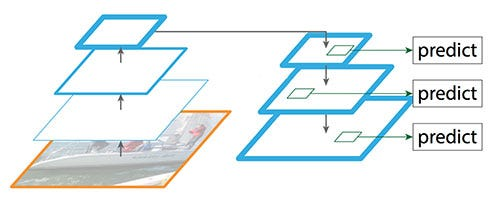
\includegraphics[height=5cm,width=9cm]{Chapitre2/img16_.jpg}
          \caption{Feature Network Pyramid (FNP)}
          \label{img16_}
          \end{figure}
     \begin{figure}[H]
          \centering
          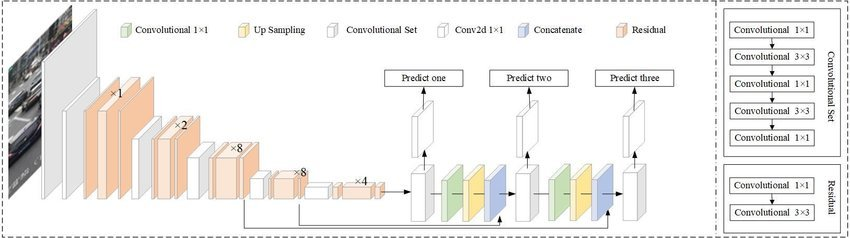
\includegraphics[height=6cm,width=14cm]{Chapitre2/img16.jpg}
          \caption{Architecture de YOLOv3}
          \label{img16}
          \end{figure}
     

\subsection{YOLOv4} 

Créé par Alexeï Bochkovski en 2020, L'architecture de YOLOv4 est composée de CSPDarknet53 en tant que colonne vertébrale, d'un module supplémentaire de regroupement de pyramides spatiales, d'un col d'agrégation de chemins PANet et d'une tête YOLOv3. CSPDarknet53 est une nouvelle dorsale qui peut améliorer la capacité d'apprentissage de CNN. Le bloc de regroupement pyramidal spatial est ajouté sur CSPDarknet53 pour augmenter le champ réceptif et séparer les caractéristiques contextuelles les plus importantes. Au lieu des réseaux pyramidaux de fonctionnalités (FPN) pour la détection d'objets utilisés dans YOLOv3.

\subsection{YOLOv5} 

Développé par ultralytics en 2020, il a été une énorme amélioration de l'accessibilité pour la détection d'objets en temps réel en raison de la transition de Darknet à PyTorck en tant que cadre de mise en œuvre, car Darknet est plus difficile à configurer et moins prêt pour la production. Cette transition a entraîné une forte augmentation du temps de formation et également du temps de prédiction avec l'accessibilité au grand écosystème de PyTorch.          
     % =========== SSD ===========
% =========== Evaluation Metrics ===========
\section{Métriques pour l'évaluation des systèmes de détection d'objets} 
Pour qu'un système de détection d'objets soit utile et ait le potentiel d'apporter une contribution significative sur le terrain, son efficacité doit être soigneusement évaluée. En outre, l'évaluation doit être effectuée à l'aide de critères généraux et connus permettant une comparaison équitable avec les méthodes existantes et une confirmation de la validité et de l'utilité du système.

Les métriques de détection d'objets servent de mesure pour évaluer les performances du modèle sur une tâche de détection d'objets. Cela nous permet également de comparer objectivement plusieurs systèmes de détection ou de les comparer à une référence. En conséquence, des compétitions importantes telles que PASCAL VOC et MSCOCO fournissent des mesures prédéfinies pour évaluer les performances de différents algorithmes de détection d'objets sur leurs ensembles de données. Dans cette section, nous expliquons les principales métriques de détection d'objets et leur interprétation.
          % =========== IoU ===========
\subsection{Intersection over Union (IoU)}
Étant donné que la tâche de classification évalue uniquement la probabilité que l'objet de classe apparaisse dans l'image, c'est une tâche simple pour un classificateur d'identifier les prédictions correctes des incorrectes. Cependant, la tâche de détection d'objet localise davantage l'objet avec une boîte englobante associée à son score de confiance correspondant pour signaler la certitude avec laquelle la boîte englobante de la classe d'objets a été détectée.

L'intersection over Union, également appelée indice de Jaccard, est une métrique d'évaluation qui quantifie la similarité entre la boîte englobante de vérité terrain  et la boîte englobante prédite pour évaluer la qualité de la boîte prédite. 

Formellement, l'IoU égale à l'intersection entre la boîte de vérité terrain et la boîte prédite sur leur union. La figure \ref{img19} montre clairement cette notion d'IoU
          \begin{figure}[H]
               \centering
               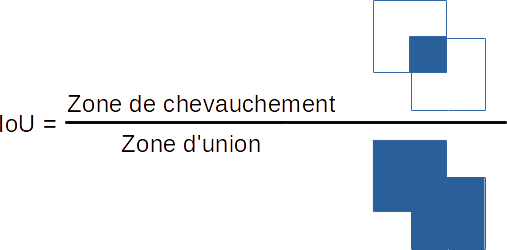
\includegraphics[height=5cm,width=10cm]{Chapitre2/img19.png}
               \caption{Intersection over Union (IoU)}
               \label{img19}
               \end{figure}

Le score IoU varie de 0 à 1, plus les deux boites englobantes sont proches, plus le score IoU est élevé (voir figure \ref{img20}.
          \begin{figure}[H]
               \centering
               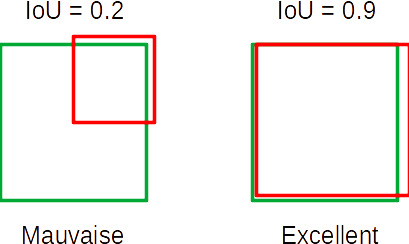
\includegraphics[height=4.5cm,width=8cm]{Chapitre2/img20.png}
               \caption{Exemples de la mesure Intersection over Union (IoU)}
               \label{img20}
               \end{figure}

          % =========== Confusion Matrix ===========
\subsection{Matrice de confusion}

En Choisissant un seuil prédéfini pour la valeur IoU, nous pouvons créer la matrice de confusion qui définit les performances d'un modèle en nous permettant de calculer d'autres mesures comme le rappel et la précision.
          \paragraph{Vrai positif (TP):} IoU >= seuil, une détection correcte. 
          \paragraph{Faux positif (FP):} IoU < seuil, une mauvaise détection.
          \paragraph{Faux négatif (FN):} Le modèle n'a pas détecté l'objet actuel.
          \paragraph{Vrai négatif (TN):} Non utilisé, il représenterait une erreur de détection corrigée. Dans la tâche de détection d'objet, il existe de nombreuses boîtes englobantes possibles qui ne doivent pas être détectées dans une image. Ainsi, TN serait toutes les boîtes englobantes possibles qui n'ont pas été correctement détectées (autant de boîtes possibles dans une image). C'est pourquoi il n'est pas utilisé par les métriques.
          \begin{figure}[H]
               \centering
               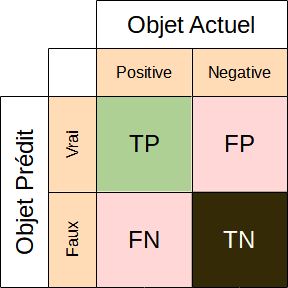
\includegraphics[height=9cm,width=9cm]{Chapitre2/mat_conf.png}
               \caption{Matrice de confusion.}
               \label{mat_conf}
               \end{figure}
          
          % =========== Precision ===========
          \subsection{Précision}
          La précision est la capacité d'un modèle à identifier uniquement les objets pertinents. C'est le pourcentage de prédictions positives correctes et est donné par :
          \begin{center} $Précision = \frac{TP}{TP + FP}$ \end{center}

          % =========== Recall ===========
          \subsection{Rappel}
          Le rappel est la capacité d'un modèle à trouver tous les cas pertinents (toutes les boîtes englobantes souhaitées). C'est le pourcentage de vrais positifs détectés parmi toutes les vérités recherchées pertinentes et est donné par:
          \begin{center} $Rappel = \frac{TP}{TP + FN}$ \end{center}
          
          % =========== Precision x Recall Curve ===========
          \subsection{Précision x Rappel courbe}
          La courbe Précision x Rappel est un bon moyen d'évaluer les performances d'un détecteur d'objets car la confiance est modifiée en traçant une courbe pour chaque classe d'objets. Un détecteur d'objet d'une classe particulière est considéré comme bon si sa précision reste élevée à mesure que le rappel augmente, ce qui signifie que si vous faites varier le seuil de confiance, la précision et le rappel seront toujours élevés. Une autre façon d'identifier un bon détecteur d'objets est de rechercher un détecteur capable d'identifier uniquement les objets pertinents (0 faux positifs = haute précision), en trouvant tous les objets recherchés (0 faux négatifs = rappel élevé).
          
          Un détecteur d'objets médiocre doit augmenter le nombre d'objets détectés (augmentation des faux positifs = précision inférieure) afin de récupérer tous les objets recherchés (rappel élevé). C'est pourquoi la courbe Précision x Rappel commence généralement par des valeurs de haute précision, diminuant à mesure que le rappel augmente.
          
          Le modèle est performant si la précision reste élevée lorsque le rappel devient élevé.
          \begin{figure}[H]
               \centering
               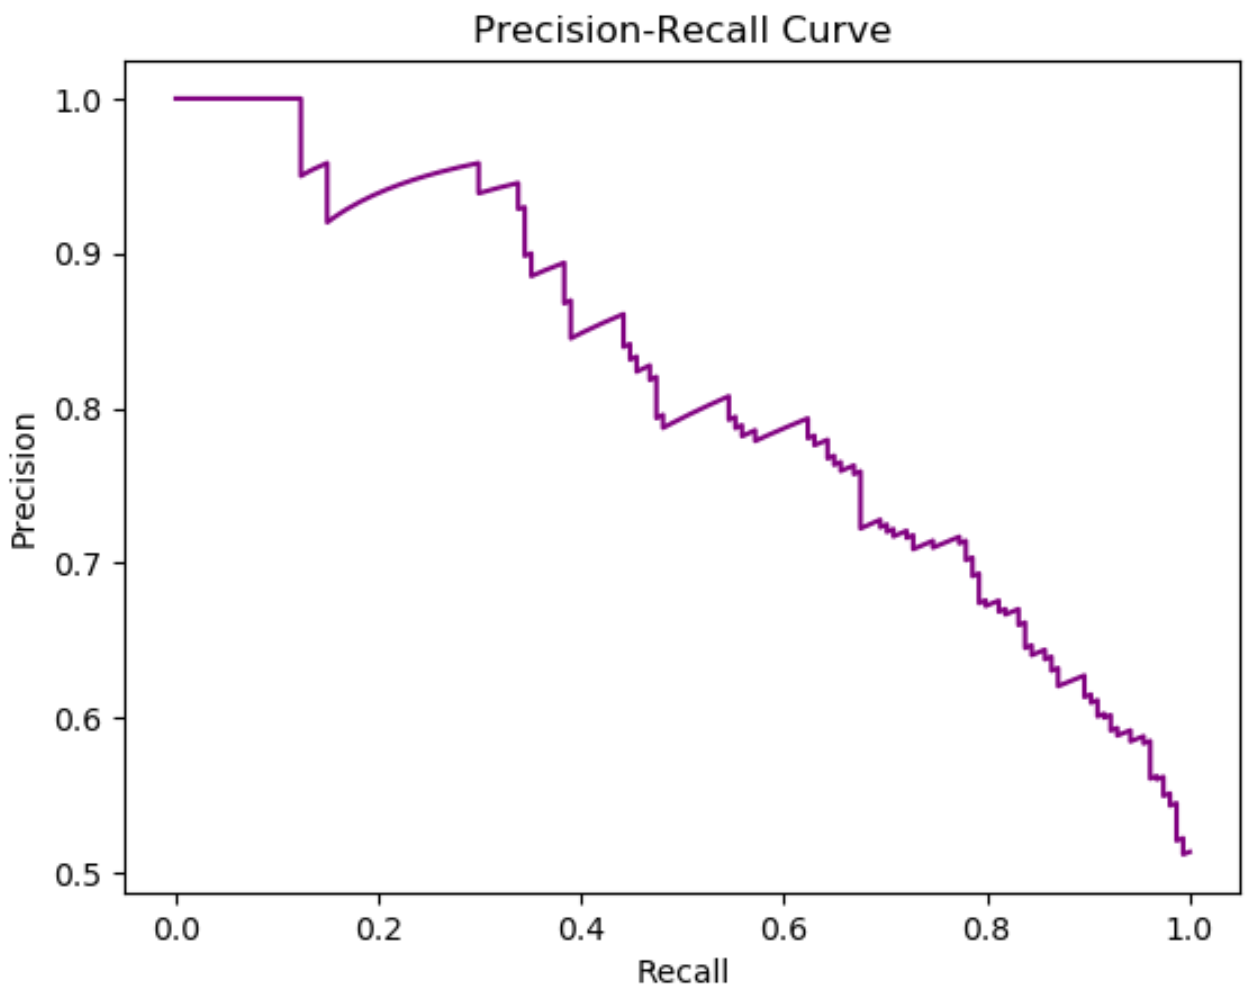
\includegraphics[height=10cm,width=12cm]{Chapitre2/img21.png}
               \caption{Exemple de Précision x Rappel courbe d'un model}
               \label{img21}
               \end{figure}
          
          % =========== AP ===========
          \subsection{Précision moyenne (AP)}
          Une autre façon de comparer les performances des détecteurs d'objets consiste à calculer l'aire sous la courbe (AUC) de la courbe Précision x Rappel. Comme les courbes AP sont souvent des courbes en zigzag qui montent et descendent, comparer différentes courbes (différents détecteurs) dans le même tracé n'est généralement pas une tâche facile car les courbes ont tendance à se croiser très fréquemment. C'est pourquoi la précision moyenne (AP), une mesure numérique, peut également nous aider à comparer différents détecteurs. En pratique, AP est la précision moyenne sur toutes les valeurs de rappel entre 0 et 1.
          
          La précision moyenne (AP) de la catégorie $C_i$ peut être calculée:
          \begin{center} $AP_{C_i} = \frac{1}{m} \sum^{m}_{j=1} P_{C_i}$ \end{center}

          % =========== mAP ===========
          \subsection{Précision moyenne moyenne  (mAP)}
          S'il existe plusieurs catégories ${C_1, C_2, ... , C_n}$ pour l'ensemble de données. Par conséquent, la précision moyenne moyenne (mAP) de l'ensemble de la catégorie peut être calculée comme suit:
          \begin{center} $mAP_{C_i} = \frac{1}{n} \sum^{n}_{j=1} P_{C_i}$ \end{center}





\section{Conclusion} 
